\documentclass[titlepage,12pt,a4paper,times]{book}

\usepackage[utf8]{inputenc}
\usepackage[portuguese]{babel}
\usepackage[T1]{fontenc}
% substituir linha anteior por 
% \usepackage[english]{babel} 
% se o relatório for escrito na língua inglesa.
\usepackage{makeidx}
\usepackage{xspace}
\usepackage{graphicx,color,times}
\usepackage{fancyhdr}
% \usepackage{pxfonts}
% \usepackage{times}
% \usepackage{mathptm}
% \usepackage{amssymb}
% \usepackage{amsfonts}
\usepackage{amsmath}
\usepackage{latexsym}
\usepackage[printonlyused]{acronym}
\usepackage{float}
\usepackage{listings}
\usepackage{tocbibind}
\usepackage{wrapfig}
\usepackage{natbib}
\usepackage{hyperref}
% \usepackage{glossaries}
% \makeglossaries

\renewcommand{\ttdefault}{phv}

\pagestyle{fancy}
\renewcommand{\chaptermark}[1]{\markboth{#1}{}}
\renewcommand{\sectionmark}[1]{\markright{\thesection\ #1}}
\fancyhf{} \fancyhead[LE,RO]{\bfseries\thepage}
\fancyhead[LO]{\bfseries\rightmark}
\fancyhead[RE]{\bfseries\leftmark}
\renewcommand{\headrulewidth}{0.5pt}
\renewcommand{\footrulewidth}{0pt}
\addtolength{\headheight}{0.5pt}
\setlength{\marginparsep}{0cm}
\setlength{\marginparwidth}{0cm}
\setlength{\marginparpush}{0cm}
\addtolength{\hoffset}{-1.0cm}
\addtolength{\oddsidemargin}{\evensidemargin}
\addtolength{\oddsidemargin}{0.5cm}
\addtolength{\evensidemargin}{-0.5cm}


% NEW COLORS
\definecolor{dark}{gray}{0.25}
\definecolor{lgray}{gray}{0.9}
\definecolor{dkblue}{rgb}{0,0.13,0.4}
\definecolor{dkgreen}{rgb}{0,0.6,0}
\definecolor{gray}{rgb}{0.5,0.5,0.5}
\definecolor{mauve}{rgb}{0.58,0,0.82}

\lstset{ %
  language=C,                    basicstyle=\footnotesize,
  numbers=none,                  numberstyle=\tiny\color{gray}, 
  stepnumber=1,                  numbersep=5pt,
  backgroundcolor=\color{white}, showspaces=false,
  showstringspaces=false,        showtabs=false,
  frame=single,                  rulecolor=\color{black},
  tabsize=2,                     captionpos=b,
  breaklines=true,               breakatwhitespace=false,
  title=\lstname,                keywordstyle=\color{blue},
  commentstyle=\color{dkgreen},  stringstyle=\color{mauve},
  escapeinside={\%*}{*)},        morekeywords={*},
  belowskip=0cm
}



\begin{document}


\thispagestyle{empty}
\setcounter{page}{-1}

\begin{center}
\begin{Huge}
\textbf{Universidade da Beira Interior}
\end{Huge}
\end{center}

\begin{center}
\begin{Huge}
Departamento de Informática
\end{Huge}
\end{center}

\vspace{0,07cm}
\begin{figure}[!htb]
\centering

\includegraphics[scale=0.3]{brasaoubi.JPG}
\end{figure}

\vspace{0.5cm}
\begin{center}
\begin{Large}
\textbf{JC1- Cristal News - Visualização e Caracterização de Notícias Web }
\end{Large}
\end{center}


\vspace{0.5cm}
\begin{center}
\begin{normalsize}
\begin{large}
Elaborado por:
\end{large}
\end{normalsize}
\end{center}

\vspace{0.2cm}
\begin{center}
\begin{large}
\textbf{Luís Carlos Durão Mata de Oliveira}
\end{large}
\end{center}

\vspace{0,5cm}
\begin{center}
\begin{normalsize}
\begin{large}
Orientador:
\end{large}
\end{normalsize}
\end{center}

\vspace{0.2cm}
\begin{center}
\begin{large}
\textbf{Professor Doutor João Paulo Cordeiro}
\end{large}
\end{center}



\vspace{0.5cm}
\begin{center}
\begin{normalsize}
9 de Julho de 2018
\end{normalsize}
\end{center}


\clearpage{\thispagestyle{empty}\cleardoublepage}

\frontmatter

\chapter*{Agradecimentos}
\label{chap:ack}

Quero agradecer desde já ao meu orientador, Professor Doutor João Paulo Cordeiro, por todo o apoio que me deu ao longo da realização do projecto, bem como a oportunidade que tive em alargar o meu conhecimento na área da interação humana com o computador.
Gostaria também de agradecer a todos os meus colegas que me apoiaram e encorajaram.
Por fim gostava de agradecer à minha família, os meus pais, José Manuel Oliveira e Maria de Lurdes Oliveira e à minha irmã, Ana Isabel Oliveira, pela educação e apoio que me deram ao longo deste caminho.

 

\clearpage{\thispagestyle{empty}\cleardoublepage}


\tableofcontents

\clearpage{\thispagestyle{empty}\cleardoublepage}

\listoffigures

% Se não existirem tabelas, comentar as seguintes linhas
\clearpage{\thispagestyle{empty}\cleardoublepage}
\listoftables

% \listoflistings

\clearpage{\thispagestyle{empty}\cleardoublepage}
\chapter*{Acrónimos}
\label{chap:acro}

\begin{acronym}[TCP]
  \acro{TCP}{Transmission Control Protocol}
\end{acronym}

\begin{acronym}[HTML]
  \acro{HTML}{Hyper Text Markup Language}
  \acro{API}{Application Programming Interface}
  \acro{MVC}{Model-view-controller}
  \acro{CSS}{Cascading Style Sheets}
\end{acronym}

% \clearpage{\pagestyle{empty}\cleardoublepage}
% \chapter*{Glossário}
\makeglossaries

\newglossaryentry{.NET Framework}
{
  name={.NET Framework},
  description={É uma plataforma para desenvolvimento e funcionamento de aplicações desenvolvida pela Microsoft.}
}

\newglossaryentry{ASP.NET}
{
  name={ASP .Net},
  description={É uma plataforma da Microsoft para o desenvolvimento de aplicações Web e é o sucessor da tecnologia ASP.}
}

\newglossaryentry{CS}
{
  name={C\#},
  description={Lê-se \textit{C Sharp} e é uma linguagem de programação orientada a objectos, desenvolvida pela Microsoft, inicialmente para a plataforma .NET. O C\# é inspirado na junção entre as linguagens C++ e Java.}
}


\newglossaryentry{Java}
{
  name={JAVA},
  description={É uma linguagem de programação orientada a objectos, desenvolvida pela Sun Microsystems na década de 90. Hoje pertence à empresa Oracle.}
}


\newglossaryentry{OpenDMTP}
{
  name={OpenDMTP},
  description={\textit{Open Device Monitoring and Tracking Protocol} é um protocolo e uma \textit{framework} abertos que permite a comunicação bidireccional entre servidores e clientes através da internet.}
}


\newglossaryentry{OpenGTS}
{
  name={Open GTS},
  description={É o primeiro projecto \textit{Open Source} \textit{Web-Based} para controlo de frotas por GPS.}
}


\newglossaryentry{VS2010}
{
  name={Visual Studio 2010},
  description={\textit{Microsoft Visual Studio 2010} é um sistema de desenvolvimento desenvolvido pela Microsoft e é dedicado ao Framework .NET, que contem um conjunto de ferramentas de desenvolvimento projectadas para auxiliar os programadores a enfrentarem desafios complexos.}
}


\newglossaryentry{WebS}
{
	name={Web Service},
	description={Web services são aplicações modulares auto-descritas e auto-contidas, que permitem a integração de sistemas e a comunicação entre aplicações de diferentes tipos.}
}


\newglossaryentry{WebBased}
{
	name={Web Based},
	description={Aplicação desenvolvida para a Web.}
}

\newglossaryentry{Roaming}
{
	name={Roaming},
	description={Define a possibilidade de um utilizador de uma determinada rede obter rede/conecção fora da área geográfica onde foi registado.}
}


\newglossaryentry{Smartphone}
{
	name={Smartphone},
	description={Smartphone é um telefone móvel que contem muitas das principais tecnologias de comunicação e serviços que existem nos computadores pessoais, como acesso a e-mails, serviços de mensagens instantâneas, internet, GPS, entre outros.}
}

\newglossaryentry{TCPIP}
{
	name={TCP/IP},
	description={É um conjunto de protocolos de comunicação entre computadores ligados rede. O nome TCP/IP surge da união entre dois protocolos: o TCP (Transmission Control Protocol) e o protocolo IP (Internet Protocol).}
}

\newglossaryentry{Firewall}
{
	name={Firewall},
	description={É o nome criado para definir um dispositivo para uma rede de computadores que tem como objectivo criar uma política de segurança num determinado ponto de controlo da rede.}
}

\newglossaryentry{JavaScript}
{
	name={JavaScript},
	description={É uma linguagem de programação baseada na linguagem de programação ECMAScript. Actualmente é a linguagem de programação mais utilizada em \textit{``Client-Side''} nos \textit{browsers}.}
}

\newglossaryentry{Flash}
{
	name={Flash},
	description={Desenvolvido pela Macromedia, o Flash é um software utilizado para criação de animações interactivas que funcionam incorporadas em \textit{Browsers}, \textit{Desktop}, \textit{Smartphones}, \textit{Tablets}, e Televisores.}
}


\newglossaryentry{StoredProcedure}
{
	name={Stored Procedure },
	description={É o nome dado a um conjunto de comandos numa base de dados de forma a simplificar a sua utilização.}
}

\newglossaryentry{SQLS}
{
	name={SQL Server 2008},
	description={É um sistema de gestão de base de dados relacional criado pela Microsoft.}
}

\newglossaryentry{Firm}
{
	name={Firmware},
	description={É o conjunto de instruções operacionais programadas directamente no \textit{hardware} de um equipamento electrónico.}
}

\newglossaryentry{browser}
{
	name={Browser},
	description={É um programa de computador que possibilita aos utilizadores uma interacção com documentos virtuais da Internet, também conhecidos como páginas Web.}
}



\clearpage{\thispagestyle{empty}\cleardoublepage}

\mainmatter
\chapter{Introdução}
Este capítulo é dedicado à apresentação do tema do projecto bem como o porque da sua escolha, vão ser apresentados os seus objectivos e  estruturação deste documento.

\label{chap:intro}

\section{Enquadramento}
\label{sec:amb} % CADA SECÇÃO DEVE TER UM LABEL
% CADA FIGURA DEVE TER UM LABEL

Atualmente o jornalismo evolui no sentido em que cada vez é mais lógico e normal investir em notícias online, com isto todos os dias são colocadas enormes quantidades de notícias novas na Internet, ficando desta forma disponíveis para milhões de pessoas.\par
Devido a este grande fluxo de notícias só temos um perceção parcial da informação noticiosa que circula nos meios eletrónicos. Assim sendo um utilizador algumas tem muitas dificuldades em encontrar as notícias em que está interessado com a facilidade que desejaria. Ele só conseguirá encontrar noticias de maior importância providenciadas pelos organizações mais relevantes.



\section{Motivação}
\label{sec:mot}
Este projeto visa a criação de uma aplicação que a partir de uma grande e variedade de notícias produz uma vista clara para os tópicos escolhidos por um utilizador. Através de uma interface atualizada em tempo real e com o maior número de notícias possíveis, de acordo com o tópico escolhido, permite ao utilizador ter uma visão abrangente sobre os temas, reduzindo o tempo de pesquisa tornando mas simples a procura de notícias.

\section{Objetivos}
\label{sec:obj}
O objectivo deste projecto passa por testar, estudar e experimentar medidas de \emph{web srcaping} de forma a sintetizar o número de notícias presentes na \emph{web}. Através de uma aplicação o utilizador terá acesso a noticias separadas por tópicos, em cada tópico será possível realçar notícias consoante um léxico de palavras escolhido pelo utilizador. 

\section{Organização do Documento}
\label{sec:organ}

De modo a refletir o trabalho que foi feito, este documento encontra-se estruturado da seguinte forma:
\begin{enumerate}
\item O primeiro capítulo -- \textbf{Introdução} -- apresenta o projeto, a motivação para a sua escolha, o enquadramento para o mesmo, os seus objetivos e a respetiva organização do documento.
\item O segundo capítulo -- \textbf{Tecnologias Utilizadas} -- descreve os conceitos mais importantes no âmbito deste projeto, bem como as tecnologias utilizadas durante do desenvolvimento da aplicação.
\item O terceiro capítulo -- \textbf{Tecnologia e Ferramentas Utilizadas} -- descreve as tecnologias utilizadas durante o desenvolvimento do projecto
\item o quarto capítulo -- \textbf{Implementação e Testes} -- apresenta e discute os resultados obtidos através do uso da aplicação desenvolvida
\item O quinto capítulo -- \textbf{Conclusões e Trabalho Futuro} -- descreve as conclusões obtidas pelo autor, bem como algumas sugestões de desenvolvimento do projecto no futuro.
\end{enumerate}

\clearpage{\thispagestyle{empty}\cleardoublepage}
\chapter{Estado da Arte}
% OU \chapter{Trabalhos Relacionados}
% OU \chapter{Engenharia de Software}
% OU \chapter{Tecnologias e Ferramentas Utilizadas}
\label{chap:estado-da-arte}

\section{Introdução}
\label{chap2:sec:intro}
O \hyperref[chap:estado-da-arte]{Capítulo 2} vai ser apresentado um modelo de redação de notícias, que se mostrou bastante útil neste projeto.

\section{Modelo pirâmide invertida}
\label{chap2:sec:...}
A notícia não é mais do que texto jornalístico relativo a um conteúdo factual e relata acontecimentos de interesse geral com a menor subjetividade possível.
O texto da notícia deve ser escrito com clareza, simplicidade e exatidão, assim como o bom uso do português e do cumprimento da gramática.
Uma notícia presente na \emph{Internet}, requer um tratamento diferente das demais, estas combinam texto som e imagem.\par
O modelo pirâmide invertida, tem uma função interessante no que diz respeito à redação de notícias, consiste em apresentar primeiro as informações mais importantes e na sequência da notícia apresentar as informações menos importantes. Isto permite ao leitor ter uma noção do que será apresentado ao longo da notícia, só através do primeiro parágrafo.

\vspace{0,07cm}
\begin{figure}[H]
\centering
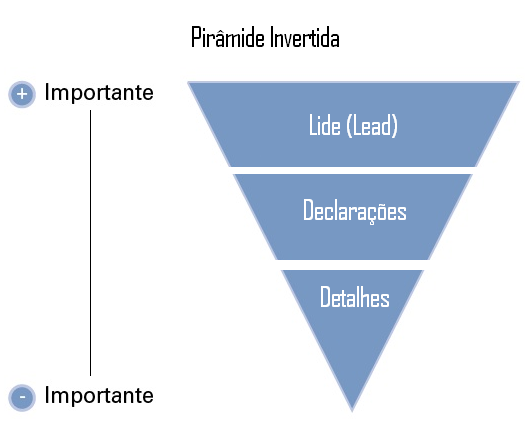
\includegraphics[scale=0.5]{relatorio-projeto/imagens/piramide_invertida.png}
\caption{Pirâmide invertida.}
\label{fig:pirâmide}
\end{figure}
 
 Na \hyperref[fig:pirâmide]{Figura 2.1} observamos que a pirâmide começa com o \emph{Lide(Lead)}, este não é mais do que a introdução da notícia. É onde se situa o leitor com os factos que aconteceram, deve conter respostas às seguintes perguntas: 'O que?', "Quando?", "Quem?", "Como?", "Onde?" e principalmente "Porque?".
 A secção \emph{Declarações} tem como objetivo desenvolver a notícia, suportando-a com informações, entrevistas ou referências.
 À medida que o notícia se desenrola os \emph{Detalhes} cada vez menos importantes por isso têm a posição mais baixa para pirâmide.
 \par
Com base neste modelo utiliza-se o primeiro parágrafo de uma notícia para ser mostrado na aplicação desenvolvida.
 

\clearpage{\thispagestyle{empty}\cleardoublepage}
\chapter{Tecnologias e Ferramentas Utilizadas}
% OU \chapter{Trabalhos Relacionados}
% OU \chapter{Engenharia de Software}
% OU \chapter{Tecnologias e Ferramentas Utilizadas}
\label{chap:tecno-ferra}

\section{Introdução}
\label{chap3:sec:intro}
O capítulo 3 é dedicado à identificação das ferramentas e tecnologias usadas para desenvolver este projeto. Foram usadas algumas das seguintes ferramentas: \emph{JavaFx} para desenvolver a interface gráfica da aplicação, a biblioteca \emph{JSOUP} uma ferramenta que permite analisar um documento \emph{HTML} e \emph{GitHub} para controlo de versões.

\section{Recursos Utilizados}
\label{chap3:sec:...}

\subsection{NetBeans}
O \emph{NetBBeans} é um ambiente de desenvolvimento de código, onde é possível desenvolver uma grande variedade de linguagens, dentro das quais \emph{Java}, usada neste projeto.
Auxilia programadores a escrever, compilar, no \emph{debug} de código e até mesmo a instalar aplicações. \par
A sua estrutura está feita de forma a simplificar o desenvolvimento e aumentar a produtividade, uma vez que reúne numa única aplicação todas as funcionalidades descritas anteriormente.\par
O \emph{NetBeans} fornece uma base sólida para a criação de projetos, possui um grande conjunto de bibliotecas e \ac{API}, além de uma documentação vasta. Isto faz com que o utilizador escreva o seu código de uma forma mais rápida. \par
Optei por escolher o \emph{NetBeans} porque já tinha experiência anterior na sua utilização e pareceu a mais adequada para usar em conjunto com o \emph{SceneBuiler}.

\subsection{SceneBuilder}
O \emph{SceneBuilder} é uma plataforma de desenvolvimento de ambientes gráficos, que permite criar rapidamente uma aplicação \emph{JavaFx}, sem recurso a código.\par 
Os utilizadores podem arrastar componentes, modificar as suas propriedades, aplicar estilos e o código \emph{FXML} é gerado automaticamente. Esse ficheiro \emph{FXML} é combinado com código \emph{Java}.\par
Permite moldar facilmente o ambiente gráfico da aplicação e adequa-lo às nossas necessidades. O código \emph{FXML} é gerado automaticamente, separadamente da interface lógica da programação. É possível abrir o ficheiro \emph{FXML} e editar o seu código.\par
A qualquer momento da criação do projeto, é possível pré-visualizar a aplicação durante o seu desenvolvimento.

\vspace{0,07cm}
\begin{figure}[H]
\centering
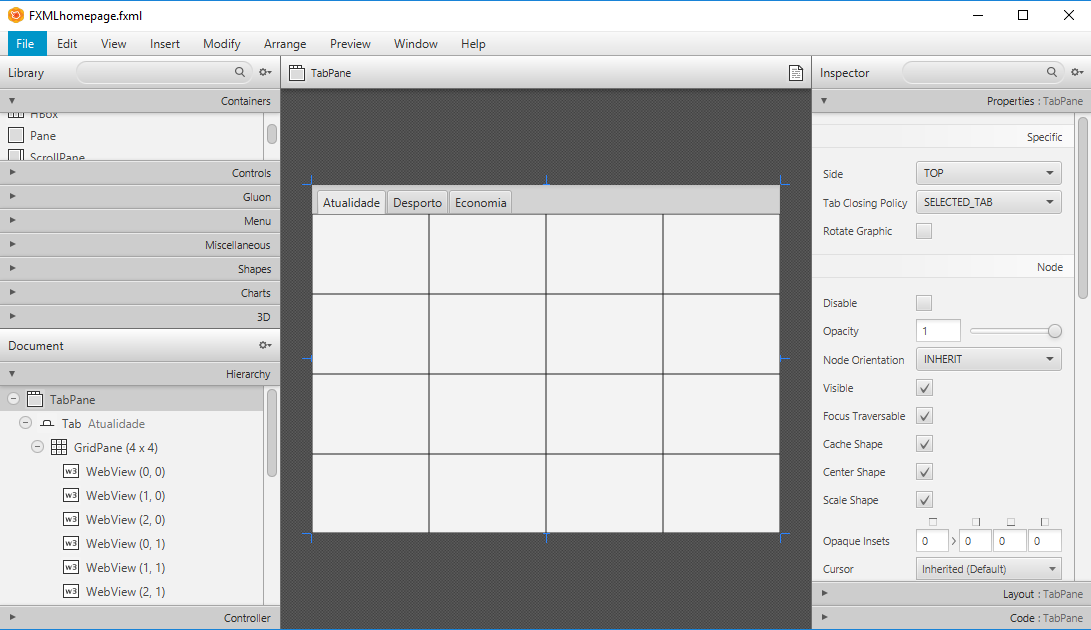
\includegraphics[scale=0.4]{imagens/scene_builder.PNG}
\caption{\emph{Scene Builder}.}
\label{fig:scenebuilder}
\end{figure}
Na figura \ref{fig:scenebuilder} é possível ver uma interface que foi desenvolvida no projeto, permitiu criar de forma rápida uma página que contem muitos elementos.
Foi usado para desenvolver o ambiente gráfico do projeto, fazendo uma ligação rápida com o código \emph{Java}.

\subsection{JavaFx}
\emph{JavaFX} é uma plataforma que permite desenvolver aplicações com interface gráfica com base na programação por eventos. Os \emph{eventos} tratam-se nada mais do que a captura de ações desencadeadas pelo utilizador, tais como, carregar num botão ou numa imagem. Quando isso acontece certos eventos são desencadeados, originando uma resposta. \par
O \emph{JavaFx} interage com o utilizador de acordo com o modelo \ac{MVC}, este consiste em dividir uma aplicação em três partes interligadas. Este modelo é usado para separar as representações internas da informação da forma como a informação é apresentada e aceite pelo utilizador.

\vspace{0,07cm}
\begin{figure}[H]
\centering
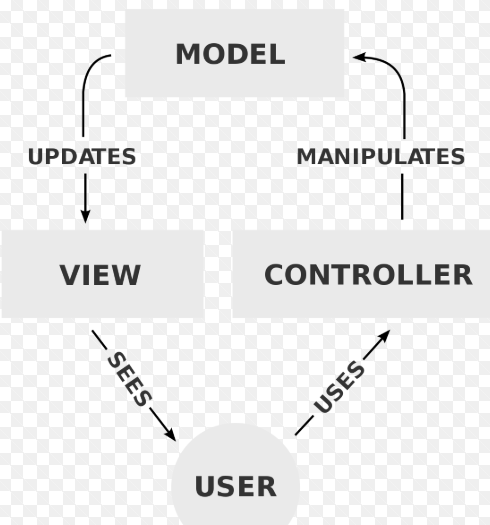
\includegraphics[scale=0.5]{imagens/mvc.PNG}
\caption{Diagrama de interacções do \ac{MVC}.}
\label{fig:gestao}
\end{figure}

Na figura 3.2 está representado o diagrama de interações do modelo \ac{MVC}. Observamos que o \emph{Model} é a componente central, é independente do utilizador e gere os dados, a lógica e regras da aplicação.
A \emph{View} pode ser qualquer representação da informação, tais como um gráfico ou um diagrama. 
A terceira parte \emph{Controller} aceita o \emph{input} e converte-o em comandos para serem interpretados pelo \emph{Model}


Em conjunto com o \emph{SceneBuilder}, o \emph{JavaFx} demonstrou ser uma excelente ferramenta para o desenvolvimento de aplicações com interface gráfica, em conjunto estas duas ferramentas foram usadas para desenvolver a seguinte interface gráfica: 

\vspace{0,07cm}
\begin{figure}[H]
\centering
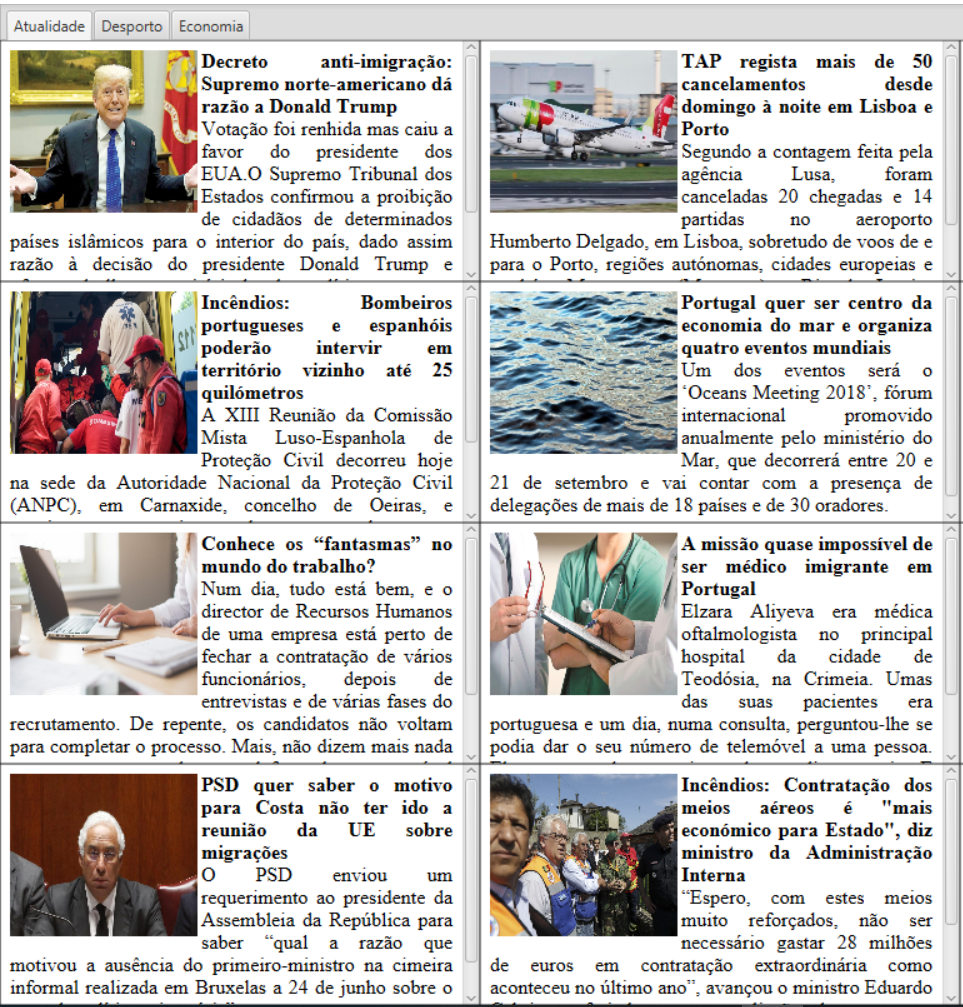
\includegraphics[scale=0.5]{imagens/app_img.png}
\caption{Imagem parcial da aplicação.}
\label{fig:gestao}
\end{figure}
A interface gráfica é particularmente simples de usar, tem como objetivo principal mostrar notícias e destacar aquelas que o utilizador considera mais importantes, através de um realçar da cor de fundo da própria notícia. Através do uso de separadores é possível escolher diferentes temas das notícias.\par
É possível atualizar as notícias carregando no botão \emph{"R"} e também são automaticamente atualizadas a cada meia hora, isto faz com que a aplicação esteja sempre atualizada.

\subsection{JSOUP}
\emph{Jsoup} é uma biblioteca \emph{Java} que permite analisar, manipular e extrair informações guardadas num documento \ac{HTML}. No âmbito deste projeto revelou-se muito importante, uma vez que através do \emph{Jsoup} que consegui manipular \emph{websites}, extraindo o seu código \ac{HTML} e a partir daí usar as informações a meu gosto.  \par 
Foram usadas várias funcionalidades do \emph{Jsoup}, tais como objetos do tipo \emph{Document},  que representam o código \ac{HTML} de uma página e objetos do tipo \emph{Element}, estes representam \emph{tags} \ac{HTML} e é a partir delas que navegamos pelo documento.

\begin{lstlisting}[language=Java, caption = Selecionar imagens de \emph{website} \label{code:imagens}]

try {
    Document document = Jsoup.connect(url).get();
    
    Elements locator = document.select("article[data-kpi] > figure > a > img");
            
    for (Element element : locator) {
        img_links.add(element.attr("src")); 
    }
    } catch (IOException e) {
        e.printStackTrace();
}
\end{lstlisting}
Na Listing 3.1 podemos observar em primeiro lugar que é feita uma conceção com o site, isto faz com que o código \ac{HTML} seja carregado para o objeto \emph{document}. \par
Pode-se observar o método \emph{select}, este permite encontrar elementos de acordo com uma \emph{query} feita ao documento.  O \emph{select} presente na imagem dá origem a todos as \emph{tags} \emph{img} que contêm a imagem de uma notícia. Considerando o código \ac{HTML} está estruturado como uma árvore, primeiro procura-se por uma \emph{tag} \emph{article} que contenha um atributo \emph{data-kpi}, a partir daqui procuram-se descendentes diretos (filhos), até encontrarmos a \emph{img} que pretendemos.
 A imagem seguinte revela exatamente o que foi descrito anteriormente.
\vspace{0,07cm}
\begin{figure}[H]
\centering
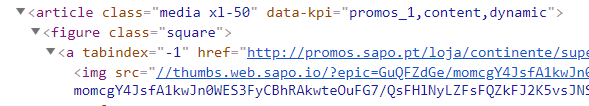
\includegraphics[scale=0.7]{imagens/html_img.PNG}
\caption{\emph{Tag img} com imagem da notícia.}
\label{fig:gestao}
\end{figure}



Este é um exemplo da utilização do \emph{Jsoup} no projeto, existem outros semelhantes que retiram o título das notícias ou o primeiro parágrafo da notícia, a técnica usado é em todo semelhante à do exemplo representado anteriormente.

\subsection{GitHub}
O \emph{GitHub} é um sistema de controlo de versões de código, através do qual  é possível realizar uma gestão mais eficaz do projeto sem correr o risco de apagar versões anteriores. Foi útil para este projeto porque permitiu guardar versões anteriores, muitas vezes ao implementar funcionalidades novas era possível testar versões anteriores em separado.
O repositório deste projecto pode ser consultado em \url{https://github.com/luisoliveira22/cristalNews.git}.


  

\section{Conclusões}
\label{chap3:sec:concs}
Neste capítulo foram descritas e caracterizadas detalhadamente as ferramentas e tecnologias usadas neste projeto, portanto, explicado o porquê da sua utilização.
\clearpage{\thispagestyle{empty}\cleardoublepage}
\chapter{Implementação e Testes}
% Os titulos dados aos capítulos são meros exemplos. Cada relatório deve adequar-se ao projeto desenvolvido.
\label{chap:imp-test}

\section{Introdução}
\label{chap4:sec:intro}
O capítulo 4 e dedicado á apresentação de algumas funções implementadas no âmbito do projeto e também alguns testes efetuados.

\section{Implementação}
\label{chap4:sec:...}

\subsection{HTML dinâmico}
Durante o desenvolvimento deste projeto, foi usada a construção dinâmica de um ficheiro \ac{HTML}, que diz respeito a uma notícia. 

\begin{lstlisting}[language=Java, caption = Exemplo de construção de \ac{HTML} dinâmico \label{code:html_dinamico}]
String html
    = "<html>"
    + "   <head>"
    + "      <style>"
    + "         p { text-align: justify;}"
    + "      </style>"
    + "   </head>"
    + "   <body bgcolor=" + "\"" + bgcolor + "\">"
    + "      <img src=" + "\"" + imagensAtualidade.get(i) + "\"" + "align=" + img_align + " width=\"150\" height=\"130\" />"
    + "      <p><b>" + titulosAtualidade.get(i) + "</b><br>"
    + paragrafosActualidade.get(i)
    + "      </p>"
    + "   </body>"
    + "</html>";
webviewActualidade[i].getEngine().loadContent(html);    

\end{lstlisting}
Neste caso foram usados métodos de \emph{Jsoup} para extrair a informação pretendida de uma página. Essas informações são armazenadas em \emph{ArrayList<String>}, e é a partir delas que se constrói o \ac{HTML}. Estão presentes três \emph{ArrayList} diferentes, \emph{imagensAtualidade, titulosAtualidade e paragrafosAtualidade}. Cada uma armazena informações em \emph{Strings} referentes às imagens, aos títulos e aos parágrafos, das noticias. \par
No fim de a \emph{string html} estar finalizada, necessitamos de mostrar o seu conteúdo. Para isso é usado um objeto do tipo \emph{WebView}, este permite exibir uma página \emph{web}, quer através do \emph{link} direto para o mesmo ou através de uma \emph{string}, o último é usado neste projeto.
Através dos métodos \emph{getEngine().loadContent(html)} é possível carregar o conteúdo da string para o \emph{webview}, neste caso se as dimensões da página forem superiores às dimensões do \emph{webview}, este cria um \emph{scroll} automático. Esta é uma propriedade bastante interessante pois em grande parte dos casos as notícias excedem o tamanho do \emph{webview}.


\subsection{DestkNew}
Esta função determina se uma notícia vai ser ou não destacada, alterando a cor de fundo da mesma. Tem como objetivo realçar uma notícia aos olhos do utilizador. 

\begin{lstlisting}[language=JAVA, caption = Código usado para destacar notícia \label{code:imagens}]
private Boolean destakNew(String texto_noticia)
HashSet<String> textNot = new HashSet<>();
String[] palavras = texto_noticia.trim().split("[ ,;:.!?\n]+");
for (String palavra : palavras) {
    textNot.add(palavra);
}

int lexSize = lexicoRelevante.size();
textNot.retainAll(lexicoRelevante);
double conjuction = (double) textNot.size() / lexSize;

if (conjuction > 0.35) {
    return true;
} else {
    return false;
}    
\end{lstlisting}

Para isso foi usado um léxico de palavras escolhido pelo utilizador, esse léxico é comparado com o texto da notícia e no final só é destacada se a interseção dos dois conjuntos for superior a 35\%. \par
Assim sendo, são usados objetos do tipo \emph{HashSet<String>}, este cria uma estrutura de \emph{string} que usa tabelas de \emph{hash} para armazenar os dados. Não permite objetos duplicados e e não segue a ordem de inserção dos dados, cada \emph{string} é identificada com um número único. \par
Na Listing 4.2 visível o \emph{lexicoRelevante}, um \emph{HashSet} que carrega as palavras de um ficheiro. Este ficheiro é manipulado pelo utilizador e deve conter palavras que ache relevantes aparecerem na notícia. Estas vão depender do seu gosto e das suas preferências. Outro \emph{HashSet} utilizado é o \emph{textNot}, que por sua vez contem as palavras presentes no parágrafo da notícia.\par 
Através do método \emph{retainAll} é feita a interseção dos dois \emph{HashSet} e a partir daqui é possível relacionar o texto da notícia com o léxico. Este método devolve apenas o conjunto de \emph{strings} comuns nos dois conjuntos de dados. Sendo o \emph{lexSize} o tamanho do \emph{lexicoRelevenate}, usado para calcular a percentagem final de quantas palavras do léxico estão presentes na notícia.
A seguinte expressão demonstra o cálculo efetuado no algoritmo:
\begin{equation}
    \mu= \dfrac{textNot \cap lexicoRelevante}{lexSize}
\end{equation}

Se ocorrer que, \begin{equation}
    \mu>35\%
\end{equation}
a notícia será destacada. Optou-se por 35\%, pois apesar de existir um léxico para cada tema, dentro do mesmo tema podem existir várias palavras que não faz sentido aparecerem  na mesma notícia.

De seguida são demonstrados alguns exemplos, atribuindo valor a cada um dos \emph{HashSet}.
\begin{table}[H]
\centering
\begin{tabular}{|c|c||c|}
\hline
\textbf{textNot} & \textbf{lexicoRelevante} & \textbf{retainAll}\\
\hline
\hline
primeiro & economia & Costa \\
\hline
ministro & parlamento &  António\\
\hline
António &  petróleo & sucesso\\
\hline
Costa &  Angola & cimeira\\
\hline
considera &  António & ministro\\
\hline
cimeira &  Costa & europeia\\
\hline
europeia &  cimeira & primeiro\\
\hline
um  & europeia&\\
\hline
sucesso &  investimento &\\
\hline
 & orçamento & \\
\hline
\end{tabular}
\caption{Exemplo de interseção de dois léxicos.}
\label{tab:exemplo}
\end{table}

Na tabela 4.1 observamos o resultado do método \emph{retainAll}, dado dois léxicos, um com a notícia e outro com o \emph{léxicoRelevante}. Podemos concluir que a notícia presente no exemplo será destacada.


\vspace{0,07cm}
\begin{figure}[H]
\centering
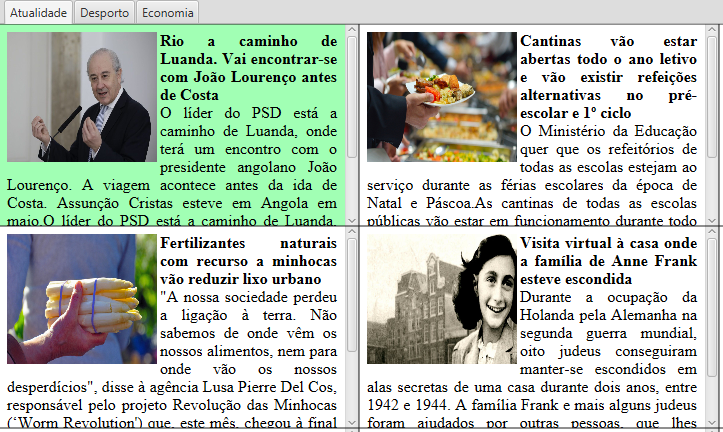
\includegraphics[scale=0.5]{imagens/new_destak.PNG}
\caption{Exemplo de notícia destacada.}
\label{fig:gestao}
\end{figure}
Na figura 4.1 é possível ver a diferença que existe para o utilizador de uma notícia que foi destacada, para as restantes. Aqui obtemos o efeito pretendido, uma vez que a notícia desperta a atenção do utilizador, sendo fácil localizar primeiro as notícias destacadas.\par



\subsection{getParagraph}
\label{chap4:sec:paragraph}
Esta função é muito relevante no contexto do projeto, uma vez que permite simplificar a notícia que será mostrada.
Para isto é usado um algoritmo bastante simples mas muito eficaz.

\begin{lstlisting}[language=JAVA, caption = Código usado para destacar notícia \label{code:getparagraph}]
Document doc = Jsoup.connect(url).get();
Elements paragrafos = doc.select("p");
StringBuilder sb = new StringBuilder();
    for (Element paragrafo : paragrafos) {
        String t = paragrafo.text().trim();
        if (t.length() == 0) {
                continue;
        }
        char last = t.charAt(t.length() - 1);
        if (".!?".contains(last + "")) {
            sb.append(t);
            if (sb.length() > 200) {
                    break;
            }
        }
    }
\end{lstlisting}
Com recurso a \emph{Jsoup} escolhe-se o primeiro parágrafo, \emph{p}, do documento \ac{HTML}. O próximo passo é escolher apenas aqueles cujo último caráter seja um dos seguintes sinais de pontuação: ., ! ou ?.
Este algoritmo é simples mas extremamente eficaz, uma vez que todos os parágrafos de uma notícia terminam com alguns destes sinais de pontuação, neste caso será guardado o primeiro parágrafo por ser considerado o que contem informações mais relevantes dentro de uma notícia. Esta seleção de parágrafos mostrou-se importante, uma vez que algumas páginas \emph{web} não usam as \emph{tags p} para mostrar os parágrafos da notícia, houve casos em que o primeiro parágrafo do \emph{website} dizia respeito ao autor do texto e não propriamente do texto da notícia.

\section{Conclusões}
\label{chap4:sec:concs}
Neste capítulo foram apresentadas algumas funções usadas, bem como o resultado da sua utilização. 
\clearpage{\thispagestyle{empty}\cleardoublepage}
\chapter{Conclusões e Trabalho Futuro}
\label{chap:conc-trab-futuro}


\section{Introdução}
Neste capítulo são apresentadas as principais conclusões sobre o trabalho desenvolvido, bem como o trabalho futuro que pode ser desenvolvido.


\section{Conclusões Principais}
\label{sec:conc-princ}
Pode-se concluir que existem métodos eficazes que permitem retirar a informação presente na \emph{web}, estes seguem regras que se mostraram eficazes.\par 
Através de experiências realizadas e implementadas, como apresentadas em \emph{getparagraph} (\ref{chap4:sec:paragraph}), provou ser um método eficaz, pois em grande parte dos \emph{websites} utilizados, foram poucos os casos em que não devolveu um parágrafo válido para a notícia.\par
Este projeto provou também que existe uma forma diferente de ver notícias, pois podem ser observadas de uma forma resumida e onde se destacam conteúdos que o utilizador considera relevantes.
 



\section{Trabalho Futuro}
\label{sec:trab-futuro}
Grande parte do trabalho futuro passa pelo estudo e desenvolvimento de novas técnicas de aceder a \emph{websites} com conteúdo noticioso. A aplicação usa o recurso ao \emph{website}, \url{www.sapo.pt}, se a  estrutura do cógido \ac{HTML} for alterada, os métodos \emph{Jsoup} necessitam de ser alterados, tais como, as \emph{querys} ao documento \ac{HTML}.
Também passará por melhorar os métodos desenvolvidos, uma vez que alguns deles são muito pesados computacionalmente, idealmente era bom usar métodos de forma a poupar recursos e aumentando a velocidade no processamento da informação.



\clearpage{\thispagestyle{empty}\cleardoublepage}

% SE EXISTIREM APENDICES, DESCOMENTAR O QUE ESTÁ EM BAIXO
% \appendix
% \include{apendice1}
% \clearpage{\pagestyle{empty}\cleardoublepage}
% \include{continuacao}
% \clearpage{\pagestyle{empty}\cleardoublepage}
% \include{apendice2}
% \clearpage{\pagestyle{empty}\cleardoublepage}
% \include{apendice3}
% \clearpage{\pagestyle{empty}\cleardoublepage}


\backmatter


\nocite{1}
\nocite{2}
\nocite{3}
\nocite{book}
\nocite{book1}
\nocite{4}

\bibliographystyle{plain}
\bibliography{bibliografia}


\end{document}